%! TeX program = pdflatex
%! TeX TS-program = pdflatex

\documentclass[10pt]{IEEEtran}
\usepackage{amsmath}
\usepackage[utf8]{inputenc}
\usepackage{fontenc}
\usepackage{dirtytalk}
\usepackage{biblatex}
\usepackage[dvipsnames]{xcolor}
\usepackage[cmintegrals]{newtxmath}
\usepackage{tikz}
\usepackage{varwidth}
\usepackage{graphicx}
\usetikzlibrary{positioning}
\tikzset{
  x=1em,
  y=1em,
}
\bibliography{bibliography}
\nocite{*}

\title{Brief history of neural networks and a perceptron implementation}

\author{ Brandon Marquez Salazar }

%! TeX program = xelatex
%! TeX TS-program = xelatex
%! TeX root = ProgramaciónEvolutiva.tex
%%%%%%%%%%%%%%%%%%%%%%%%%%%%%%%%%%%%%%%%%%%%%%%%%%%%%%%%%%%%%%%%%%%%%%%%
% Define AntiqueWhite color
\definecolor{AntiqueWhite}{RGB}{250,235,215}
\definecolor{mypurple}{RGB}{104,020,108}
\setbeamercolor*{palette primary}{use=structure,fg=white,bg=mypurple}
\setbeamercolor{normal text}{fg=white, bg=black}
\setbeamercolor{tcolorbox text}{fg=white, bg=black}
\setbeamertemplate{navigation symbols}{}                              %
\newcommand{\colouredcircle}{%
  \tikz{\useasboundingbox (-0.2em,-0.32em) rectangle(0.2em,0.32em);
        \draw[ball color=PineGreen!7!Plum!90!Red,shading=ball,line width=0.03em] (0,0) circle(0.18em);}}
\newcommand{\colouredcircledis}{%
  \tikz{\useasboundingbox (-0.2em,-0.32em) rectangle(0.2em,0.32em);
        \draw[ball color=PineGreen!7!Plum!20!Black,shading=ball,line width=0.03em] (0,0) circle(0.18em);}}
\setbeamertemplate{itemize item}{\colouredcircle}
\setbeamercolor*{bibliography entry title}{fg=Yellow!80!White, bg=Black}
% Set beamer bibliography titles and numbers color to antique white
\setbeamercolor*{bibliography entry author}{fg=AntiqueWhite}
\setbeamercolor*{bibliography entry location}{fg=AntiqueWhite}
\setbeamercolor*{bibliography entry note}{fg=AntiqueWhite}
%% Numbering color to Pine Green
\setbeamercolor*{bibliography item}{fg=LimeGreen!80!White}
% Set beamer bibliography urls color to some magenta
\setbeamercolor*{bibliography entry url}{fg=Magenta}
% Captions color to rgba (0,255,0,1)
\definecolor{LimeGreen}{RGB}{0,255,0}
\setbeamercolor{caption name}{fg=LimeGreen}
%%%%%%%%%%%%%%%%%%%%%%%%%%%%%%%%%%%%%%%%%%%%%%%%%%%%%%%%%%%%%%%%%%%%%%%%
\usepackage{tikzpagenodes}
\setbeamertemplate{background canvas}{%
  \begin{tikzpicture}[inner sep=0pt,remember picture,overlay]
    \node at (current page.center) {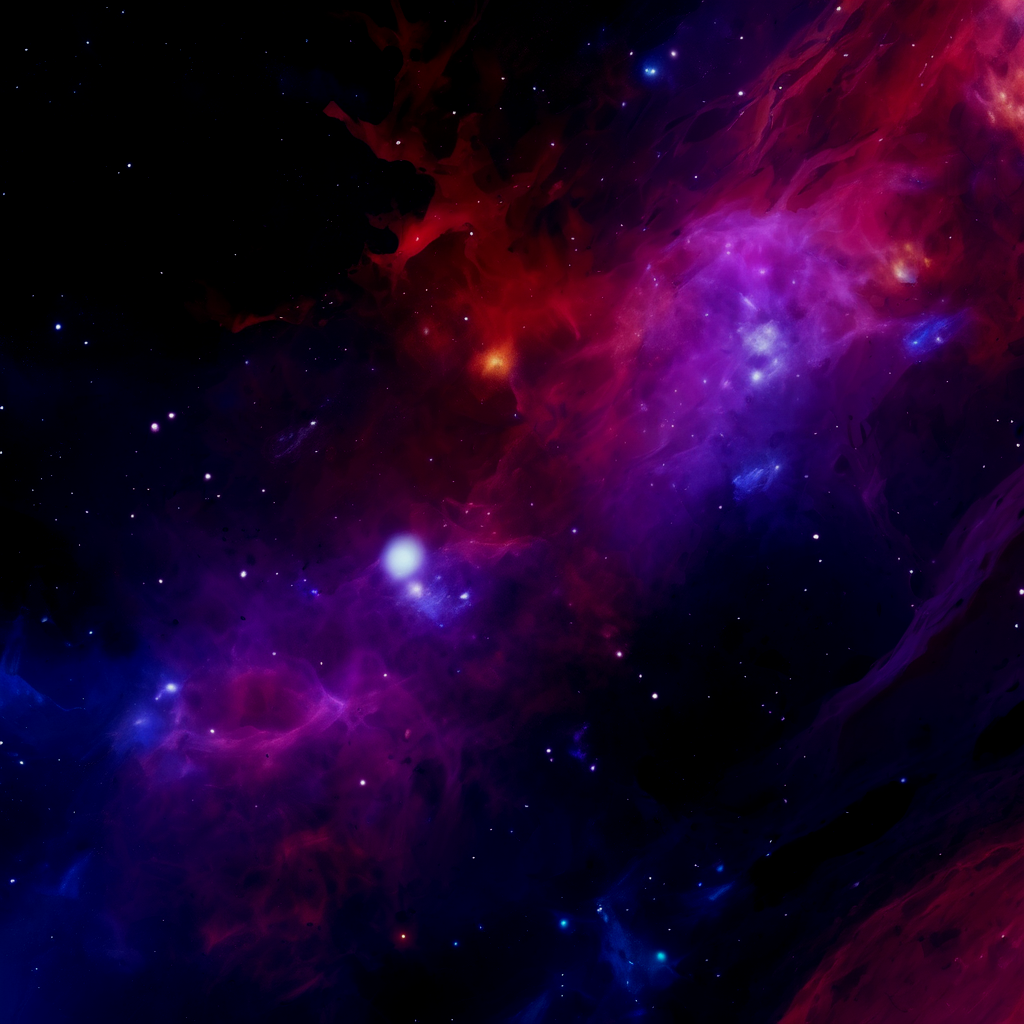
\includegraphics[height=\paperheight,width=\paperwidth]{fondo}};
  \end{tikzpicture}
}%
\usetikzlibrary{arrows.meta, decorations.pathmorphing,positioning,trees}

\lstset{
    basicstyle=\ttfamily\small,
    breaklines=true,
    backgroundcolor=\color{black!98},
    keywordstyle=\color{Magenta},
    commentstyle=\color{AntiqueWhite},
    stringstyle=\color{Yellow!80!white},
    showstringspaces=false,
    frame=single,
    rulecolor=\color{mypurple},
    frameround=tttt,
    escapeinside={\%*}{*)}
}

\makeatletter
% Set victor mono as default ttfont
\newtcolorbox{blur}[1][]{%
  #1,
  enhanced,
  remember,
  breakable, % Already enabled (good!)
  frame hidden,
  interior hidden,
  fonttitle=\bfseries\centering, 
  fontupper=\rmfamily\selectfont,
  coltext=white,
  underlay={
    \begin{tcbclipframe}
      \begin{scope}[inner sep=0pt,remember picture,overlay]
        \fill[white] (frame.south west) rectangle (frame.north east); % Changed to `frame` (not `current page`)
        \node[opacity=1] at (frame.center) {
\includegraphics[height=\paperheight, width=\paperwidth]{blured}};
      \end{scope}
    \end{tcbclipframe}
  }
}
\makeatother
%%%%%%%%%%%%%%%%%%%%%%%%%%%%%%%%%%%%%%%%%%%%%%%%%%%%%%%%%%%%%%%%%%%%%%%%
\newcommand{\separador}[1]{
  \vskip-4pt
  \begin{center}
    \rule{0.9\linewidth}{#1}
  \end{center}
}

\lstset{
  basicstyle=\ttfamily,
  showstringspaces=false,
  breaklines=true
}

\newcommand{\transparencia}[1]{%
  \begin{frame}
    \begin{blur}
      #1
    \end{blur}
  \end{frame}
}

% set bibliography background for text to be legible despite the background

\usepackage{etoolbox}
\newcommand{\setupblurbibliography}{%
  \pretocmd{\frametitle}{\blurbackground}{}{}%
  \setbeamertemplate{bibliography item}{\color{LimeGreen!80!White}\insertbiblabel}%
  \setbeamercolor{bibliography entry author}{fg=AntiqueWhite}%
  \setbeamercolor{bibliography entry title}{fg=Yellow!80!White}%
  \setbeamercolor{bibliography entry location}{fg=AntiqueWhite}%
  \setbeamercolor{bibliography entry note}{fg=AntiqueWhite}%
  \setbeamercolor{bibliography entry url}{fg=Magenta}%
}

\newtcblisting{beamerlst}[1][]{
    enhanced,
    breakable,
    listing only,
    listing options={
        style=beamerlisting,
        language=Python, % Default language
        #1
    },
    colback=black!85, % Matches your theme
    colframe=mypurple, % Your purple color
    fontupper=\ttfamily\small,
    arc=3mm, % Rounded corners
    boxrule=1pt,
    % Blur effect (optional):
    underlay={
        \begin{tcbclipframe}
        \fill[black!90] (frame.south west) rectangle (frame.north east);
        \node[opacity=0.6] at (frame.center) 
            {
\includegraphics[width=\linewidth]{blured}};
        \end{tcbclipframe}
    }
}

% Supporting style definition
\lstdefinestyle{beamerlisting}{
    basicstyle=\ttfamily\footnotesize\color{white},
    keywordstyle=\color{Magenta},
    commentstyle=\color{AntiqueWhite},
    stringstyle=\color{Yellow!80!white},
    showstringspaces=false,
    breaklines=true,
    tabsize=2
}

\newcommand{\codebox}[2][]{%
    \begin{tcolorbox}[
        enhanced,
        colback=black!85,
        colframe=mypurple,
        arc=3mm,
        boxrule=1pt,
        #1
    ]
    \lstinputlisting{#2}
    \end{tcolorbox}%
}

% Smart blur background that works with frame breaks
\newcommand{\blurbackground}{%
  \begin{tikzpicture}[remember picture,overlay]
    % Calculate content area with margins
    \path ([xshift=1cm,yshift=-1cm]current page.north west) coordinate (top left);
    \path ([xshift=-1cm,yshift=1cm]current page.south east) coordinate (bottom right);
    
    % Frosted glass effect
    \fill[black!85,opacity=0.92] (top left) rectangle (bottom right);
    \node[opacity=0.8] at (current page.center) 
      {
\includegraphics[width=\paperwidth-2cm,height=\paperheight-2cm]{blured}};
  \end{tikzpicture}%
}


\includeonly{01.-EvolutionaryComputing}

\bibliography{bibliografia}
\nocite{*}


\begin{document}
\maketitle

\section{Introduction}

There are several applications for Neural Networks nowadays and seems to
be a new technology made no so much ago, but it's origins can be found
between 1897 and 1904. When Santiago Ramón y Cajal published
\say{\textit{Histologie du système nerveux de l’homme et des vertébrés}}
where brain cells were mentioned and described as the basic element of the
nervous system; starting a new interest and acceptance over the
\say{Neuron Doctrine} extending itself into ANN investigation.


\section{Mathematical model of the neuron}

With the \say{Neuron Doctrine} popularity the need of knowledge of
neuron's inner behaviour inspired the creation of models intended to
comprehend the electrical communication from electrical excitation to
signal sending.

In 1943 McCulloch and Pitts \cite{MCCULLOCH199099} proposed the first
model of a neuron described as a binary element with different weighed
inputs $x_k w_k$ whose sum added to the bias (threshold) $\theta$ is
evaluated by a nonlinear function $S(\cdot)$ called activation function or
transfer function and giving the \say{desired} output $O$.

So, for any $j$-th neuron, the
mathematical representation is given by the following expression.

\begin{equation}
  O_j=S\left( \sum_{k=1}^{n} w_{jk} \; x_{jk}-\theta \right)
\end{equation}

Graphically we can represent it by the following scheme.

\begin{figure}[!ht]
  \centering%
  \begin{tikzpicture}
  \node (net) at ( 5, 0) [neuron] {$\sum$};
  \node (X_1) at ( 0, 4) [ninput] {$x_1$};
  \node (X_2) at ( 0, 2) [ninput] {$x_2$};
  \node (X_3) at ( 0, 0) [ninput] {$x_3$};
  \node (X_4) at ( 0,-2) [ninput] {$\cvdots$};
  \node (X_n) at ( 0,-4) [ninput] {$x_n$};
  \node (a_f) at (10, 0) [actfun] {$S(\cdot)$};
  \node (bas) at (10,-3)          {$-\theta$};
  \node (ext) at (15,0)           {$O$};
  \draw (X_1) [->] -- node[above] {$w_1$}    (2.5, 4) -- (net);
  \draw (X_2) [->] -- node[above] {$w_2$}    (2.5, 2) -- (net);
  \draw (X_3) [->] -- node[above] {$w_3$}    (2.5, 0) -- (net);
  \draw (X_4) [->] -- node[above] {$\cvdots$}(2.5,-2) -- (net);
  \draw (X_n) [->] -- node[above] {$w_n$}    (2.5,-4) -- (net);
  \draw (net) [->] --                                    (a_f);
  \draw (bas) [->] --                                    (a_f);
  \draw (a_f) [->] --                                    (ext);
  \end{tikzpicture}
  \caption{First neuron model.}%
  \label{fig::perceptron_i}%
\end{figure}


\section{The first perceptron}

The first algorithm based on the neuron model was made in 1958 and its
implementation was conceived with the \say{Perceptron Mark I} by
Rosenblatt. This algorithm was made for image recognition using
potentiometers, and motors to modify each potentiometer's value.

\begin{figure}[!ht]
  \centering%
  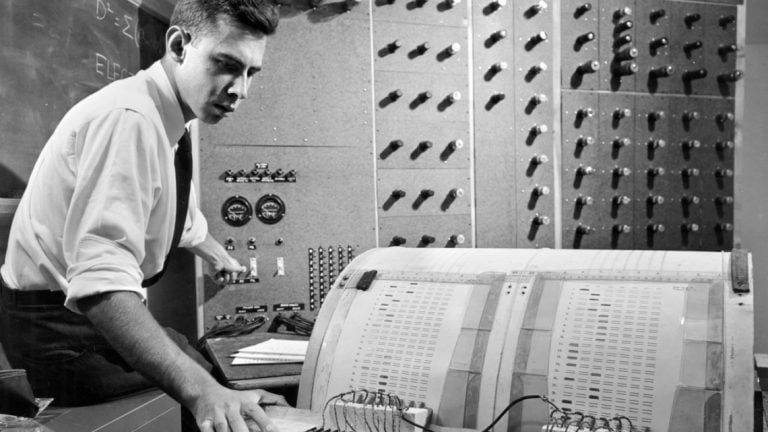
\includegraphics[width=0.8\linewidth]{img/PerceptronRosenblatt}
  \caption{In 1957, Frank Rosenblatt built the Mark I Perceptron at the
  Cornell Aeronautical Laboratory \cite{PARULAMUSTREAD}.}
  \label{RosenPerceptronMKI}
\end{figure}

\subsection{The perceptron algorithm}

Suppose any desired output $Y_j$ for the $j$-th neuron, and for each
iteration $t$ the algorithm follows the operations below:

\begin{align}
  O_j(t) &= \sign\left(\sum^{n}_{k=1} w_k(t) x_{jk}\right)
  \label{eqnOut} \\
  \epsilon_j(t)  &= \frac{\sum_{1}^{n} \left| Y_j - O_j(t) \right|}{N}
  \label{eqnErr} \\
  w_j(t+1) &\longleftarrow w_j(t) - \left(Y_j - O_j(t)\right)r
  \label{eqnWei}
\end{align}

Where Eq. \ref{eqnOut} the output, Eq. \ref{eqnErr} computes the error and
Eq. \ref{eqnWei} the weights update at iteration $t$.

\begin{figure}[!ht]
  \small%
  \centering%
  \begin{tikzpicture}
    \node [term] (st)
      {inicio};
    \node [proc,join] (pr1)
      { Initialize all $w_j$ near to $0$ };
    \node [proc,join] (pr2)
      { Evaluate $O_j$ };
    \node [proc, right=12 of st] (pr3)
      { Update all $w_j$ };
    \node [proc,join]
      { Evaluate $\epsilon_j$ };
    \node [test,join] (cd1)
      { $\epsilon_j \leq \epsilon$};
    \node [term,join]
      {fin};
    \node [coord]                   (rp1) at ($(pr1.east)!0.5!(pr3.west)$) {};
    \node [coord,right = 3 of pr3]  (rp2) {};
    \draw [cong]  (cd1) -| (rp2) -- (pr3);
    \draw [norm]  (pr2) -| (rp1) |- (pr3);
  \end{tikzpicture}
  \caption{Flowchart that describes Rosenblatt's perceptron algorithm.}
  \label{flowchart_perceptron}
\end{figure}

Something important to keep in mind it that it's convergence depends on
that the classes should be linearly separables.


\subsection{Activation, update and error functions}

During this period, and until today, there are different approaches to
neural network implementations trying to optimize it's learning, and
classifying performance.

Adaline (ADAptive Linear Neuron Element) is a neural network developed by
Widrow and Hoff, which was mainly for noise reduction, adaptive filtering,
echo reduction, among other applications. Widrow and Hoff proposed LMS
(Least Mean Squares) algorithm.

About activation functions, there are different activation functions we
can use, such as \textbf{sign}, \textbf{sigmoid}, \textbf{gaussian}, etc.
Also, some functions were defined in the search of the less loss
activation functions such as \textbf{ReLU}.


\section{A perceptrion implementation}

The implementation will be reported in the complement implemented by
Quarto \cite{QUARTOWELCOME,QUARTOGUIDE,QUARTODOCUMENTATION}, which you can
find aside this document.

The code is not optimized in order to get a legible representation of each
part described here.


\printbibliography%

\end{document}
